\documentclass{book}
\usepackage[a4paper,top=2.5cm,bottom=2.5cm,left=2.5cm,right=2.5cm]{geometry}
\usepackage{makeidx}
\usepackage{natbib}
\usepackage{graphicx}
\usepackage{multicol}
\usepackage{float}
\usepackage{listings}
\usepackage{color}
\usepackage{ifthen}
\usepackage[table]{xcolor}
\usepackage{textcomp}
\usepackage{alltt}
\usepackage{ifpdf}
\ifpdf
\usepackage[pdftex,
            pagebackref=true,
            colorlinks=true,
            linkcolor=blue,
            unicode
           ]{hyperref}
\else
\usepackage[ps2pdf,
            pagebackref=true,
            colorlinks=true,
            linkcolor=blue,
            unicode
           ]{hyperref}
\usepackage{pspicture}
\fi
\usepackage[utf8]{inputenc}
\usepackage[spanish]{babel}
\usepackage{mathptmx}
\usepackage[scaled=.90]{helvet}
\usepackage{courier}
\usepackage{sectsty}
\usepackage{amssymb}
\usepackage[titles]{tocloft}
\usepackage{doxygen}
\lstset{language=C++,inputencoding=utf8,basicstyle=\footnotesize,breaklines=true,breakatwhitespace=true,tabsize=2,numbers=left }
\makeindex
\setcounter{tocdepth}{3}
\renewcommand{\footrulewidth}{0.4pt}
\renewcommand{\familydefault}{\sfdefault}
\hfuzz=15pt
\setlength{\emergencystretch}{15pt}
\hbadness=750
\tolerance=750
\begin{document}
\hypersetup{pageanchor=false,citecolor=blue}
\begin{titlepage}
\vspace*{7cm}
\begin{center}
{\Large Laboratorio de P\-R\-O2. Ejercicio Factor P\-S\-I \\[1ex]\large version oct-\/2013 }\\
\vspace*{1cm}
{\large Generado por Doxygen 1.8.2}\\
\vspace*{0.5cm}
{\small Martes, 17 de Marzo de 2015 18:11:05}\\
\end{center}
\end{titlepage}
\clearemptydoublepage
\pagenumbering{roman}
\tableofcontents
\clearemptydoublepage
\pagenumbering{arabic}
\hypersetup{pageanchor=true,citecolor=blue}
\chapter{Ejemplo de diseño modular\-: Factor Psi.}
\label{index}\hypertarget{index}{}En este ejemplo se construye un programa modular que, dado un texto marcado, obtiene la frecuencia de la palabra más frecuente del mismo. Se introducen las clases {\itshape  Palabra} y {\itshape  Lista\-Palabras}. 
\chapter{Indice de archivos}
\section{Lista de archivos}
Lista de todos los archivos documentados y con descripciones breves\+:\begin{DoxyCompactList}
\item\contentsline{section}{src/\hyperlink{_agenda_8hh}{Agenda.\+hh} \\*Classe \hyperlink{class_agenda}{Agenda} }{\pageref{_agenda_8hh}}{}
\item\contentsline{section}{src/\hyperlink{comanda_8hh}{comanda.\+hh} \\*Classe \hyperlink{class_comanda}{Comanda} }{\pageref{comanda_8hh}}{}
\item\contentsline{section}{src/\hyperlink{_event_8cc}{Event.\+cc} \\*Classe \hyperlink{_event_8cc}{Event.\+cc} }{\pageref{_event_8cc}}{}
\item\contentsline{section}{src/\hyperlink{_event_8hh}{Event.\+hh} \\*Classe \hyperlink{_event_8hh}{Event.\+hh} }{\pageref{_event_8hh}}{}
\item\contentsline{section}{src/\hyperlink{_rellotge_8cc}{Rellotge.\+cc} \\*Metodes de \hyperlink{class_rellotge}{Rellotge} }{\pageref{_rellotge_8cc}}{}
\item\contentsline{section}{src/\hyperlink{_rellotge_8hh}{Rellotge.\+hh} \\*Classe \hyperlink{class_rellotge}{Rellotge} }{\pageref{_rellotge_8hh}}{}
\item\contentsline{section}{src/\hyperlink{_tag_8cc}{Tag.\+cc} \\*Classe \hyperlink{class_tag}{Tag} }{\pageref{_tag_8cc}}{}
\item\contentsline{section}{src/\hyperlink{_tag_8hh}{Tag.\+hh} \\*Classe \hyperlink{class_tag}{Tag} }{\pageref{_tag_8hh}}{}
\item\contentsline{section}{src/\hyperlink{token_8hh}{token.\+hh} \\*Classe \hyperlink{class_token}{Token} }{\pageref{token_8hh}}{}
\end{DoxyCompactList}

\chapter{Documentación de archivos}
\hypertarget{pro2__s52_8cc}{\section{Referencia del Archivo pro2\-\_\-s52.\-cc}
\label{pro2__s52_8cc}\index{pro2\-\_\-s52.\-cc@{pro2\-\_\-s52.\-cc}}
}


Programa principal para el ejercicio {\itshape Factor Psi}.  


Dependencia gráfica adjunta para pro2\-\_\-s52.\-cc\-:
\nopagebreak
\begin{figure}[H]
\begin{center}
\leavevmode
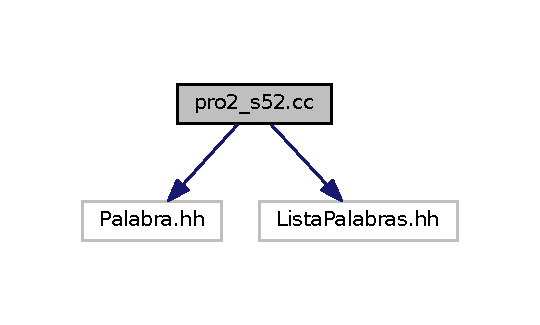
\includegraphics[width=259pt]{pro2__s52_8cc__incl}
\end{center}
\end{figure}
\subsection*{Funciones}
\begin{DoxyCompactItemize}
\item 
int \hyperlink{pro2__s52_8cc_ae66f6b31b5ad750f1fe042a706a4e3d4}{main} ()
\begin{DoxyCompactList}\small\item\em Programa principal para el ejercicio {\itshape Factor Psi}. \end{DoxyCompactList}\end{DoxyCompactItemize}


\subsection{Descripción detallada}
Programa principal para el ejercicio {\itshape Factor Psi}. 

Definición en el archivo \hyperlink{pro2__s52_8cc_source}{pro2\-\_\-s52.\-cc}.



\subsection{Documentación de las funciones}
\hypertarget{pro2__s52_8cc_ae66f6b31b5ad750f1fe042a706a4e3d4}{\index{pro2\-\_\-s52.\-cc@{pro2\-\_\-s52.\-cc}!main@{main}}
\index{main@{main}!pro2_s52.cc@{pro2\-\_\-s52.\-cc}}
\subsubsection[{main}]{\setlength{\rightskip}{0pt plus 5cm}int main (
\begin{DoxyParamCaption}
{}
\end{DoxyParamCaption}
)}}\label{pro2__s52_8cc_ae66f6b31b5ad750f1fe042a706a4e3d4}


Programa principal para el ejercicio {\itshape Factor Psi}. 



Definición en la línea 19 del archivo pro2\-\_\-s52.\-cc.


\begin{DoxyCode}
\{

\}
\end{DoxyCode}

\addcontentsline{toc}{part}{Índice}
\printindex
\end{document}
